\documentclass{article}

% Language setting
% Replace `english' with e.g. `spanish' to change the document language
\usepackage[english]{babel}

% Set page size and margins
% Replace `letterpaper' with `a4paper' for UK/EU standard size
\usepackage[letterpaper,top=2cm,bottom=2cm,left=3cm,right=3cm,marginparwidth=1.75cm]{geometry}
\usepackage{CJKutf8}
% Useful packages
\usepackage{amsmath}
\usepackage{graphicx}
\usepackage{setspace}
\usepackage{float}
\usepackage{subfigure}
\usepackage[section]{placeins}
\usepackage[colorlinks=true, allcolors=blue]{hyperref}
\usepackage[export]{adjustbox}
\usepackage{array}

\author{B10209040 陳彥倫}

\begin{document}
\thispagestyle{empty}
\hfill {\scshape \large Statistics with Meteorological Applications, Spring 2024} \hfill {\scshape P1}
\smallskip
\hrule
\begin{CJK*}{UTF8}{bsmi}
\bigskip
\bigskip
\bigskip

\centerline{\huge \textbf {HW2}}
\bigskip
\centerline{\textbf {B10209040 陳彥倫}}

\section*{1.1}
\renewcommand{\arraystretch}{1.5} 
    \begin{table}[htbp]
        \centering
        \resizebox{.5\textwidth}{!}{
        \begin{tabular}{|c|c|c|}
            \hline
            & Taipei  & Taitung \\
            \hline
            1960s & 28.80$^{\circ}$c & 27.65$^{\circ}$c \\
            2000s & 29.85$^{\circ}$c & 29.34$^{\circ}$c \\
            \hline
            \end{tabular}}
            \caption{Mean Ts for the two stations in the two periods.}
    \end{table}
\renewcommand{\arraystretch}{1.0} 

\section*{1.2}
\renewcommand{\arraystretch}{1.5} 
    \begin{table}[htbp]
        \centering
        \resizebox{.75\textwidth}{!}{
        \begin{tabular}{|c|c|c|}
            \hline
            & Taipei  & Taitung \\
            \hline
            1960s & 33.61$^{\circ}$c/25.24$^{\circ}$c & 30.94$^{\circ}$c/24.87$^{\circ}$c \\
            2000s & 33.82$^{\circ}$c/26.53$^{\circ}$c & 31.80$^{\circ}$c/26.26$^{\circ}$c \\
            \hline
            \end{tabular}}
            \caption{Mean max and min Ts.}
    \end{table}
\renewcommand{\arraystretch}{1.0} 

\section*{1.3}
\renewcommand{\arraystretch}{1.5} 
    \begin{table}[htbp]
        \centering
        \resizebox{.7\textwidth}{!}{
        \begin{tabular}{|c|c|c|}
            \hline
            & Taipei  & Taitung \\
            \hline
            1960s & 8.37$^{\circ}$c/9.53$^{\circ}$c$^2$ & 6.07$^{\circ}$c/6.92$^{\circ}$c$^2$ \\
            2000s & 7.30$^{\circ}$c/6.89$^{\circ}$c$^2$ & 5.55$^{\circ}$c/5.22$^{\circ}$c$^2$ \\
            \hline
            \end{tabular}}
            \caption{Mean DTR and variance.}
    \end{table}
    \renewcommand{\arraystretch}{1.0} 

    \newpage

\thispagestyle{empty}
\hfill {\scshape \large Statistics with Meteorological Applications, Spring 2024} \hfill {\scshape P2}
\smallskip
\hrule
\bigskip
\bigskip
\bigskip

\subsection*{Discussion}
\begin{spacing}{2}
    \begin{large}
        由Table 3的結果我們可以看出在此案例中,較大的每日最高溫及最低溫差大致上也代表著資料擁有較大的變異數。但變異數代表
        的涵義為資料分布的離散程度,因此我們也須考量資料的特性以思考各個統計度量的關聯。如氣象資料可能因測量器材及環境因素
        使得較常有離群值的產生,而此變化皆會對上述兩者造成影響。
    \end{large}
\end{spacing}



\section*{1.4}
\begin{figure}[htbp]
    \centering
    \begin{minipage}[t]{0.7\textwidth}
        \centering
        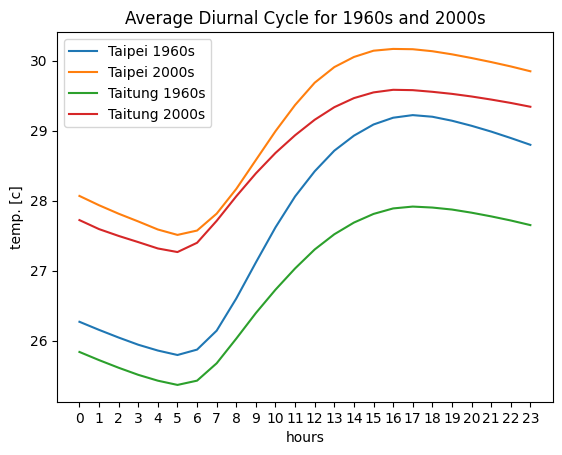
\includegraphics[width=10.5cm]{output.png}
        \caption{}
        \end{minipage}
\end{figure}

\subsection*{}
\begin{spacing}{2}
    \begin{large}
        藉由圖表比較四個不同時空背景下每日時間點的平均溫度,可以驗證隨著時間氣溫有逐漸變暖的趨勢,且台北氣溫普遍高於台東地區。
        每日最高溫及最低溫方面,可以看出最低溫皆落在早上5點,而最高溫根據時間及地點的不同,出現在下午3點到5點的區間。隨著年代
        演進,每日最高溫出現時間漸漸提前。
    \end{large}
\end{spacing}

\end{CJK*}
\end{document}